%%
%% This is file `sample-lualatex.tex',
%% generated with the docstrip utility.
%%
%% The original source files were:
%%
%% samples.dtx  (with options: `sigconf')
%% 
%% IMPORTANT NOTICE:
%% 
%% For the copyright see the source file.
%% 
%% Any modified versions of this file must be renamed
%% with new filenames distinct from sample-lualatex.tex.
%% 
%% For distribution of the original source see the terms
%% for copying and modification in the file samples.dtx.
%% 
%% This generated file may be distributed as long as the
%% original source files, as listed above, are part of the
%% same distribution. (The sources need not necessarily be
%% in the same archive or directory.)
%%
%% Commands for TeXCount
%TC:macro \cite [option:text,text]
%TC:macro \citep [option:text,text]
%TC:macro \citet [option:text,text]
%TC:envir table 0 1
%TC:envir table* 0 1
%TC:envir tabular [ignore] word
%TC:envir displaymath 0 word
%TC:envir math 0 word
%TC:envir comment 0 0
%%
%%
%% The first command in your LaTeX source must be the \documentclass command.
\documentclass[sigconf]{acmart}
%% NOTE that a single column version is required for 
%% submission and peer review. This can be done by changing
%% the \doucmentclass[...]{acmart} in this template to 
%% \documentclass[manuscript,screen]{acmart}
%% 
%% To ensure 100% compatibility, please check the white list of
%% approved LaTeX packages to be used with the Master Article Template at
%% https://www.acm.org/publications/taps/whitelist-of-latex-packages 
%% before creating your document. The white list page provides 
%% information on how to submit additional LaTeX packages for 
%% review and adoption.
%% Fonts used in the template cannot be substituted; margin 
%% adjustments are not allowed.

%%
%% \BibTeX command to typeset BibTeX logo in the docs
\AtBeginDocument{%
  \providecommand\BibTeX{{%
    \normalfont B\kern-0.5em{\scshape i\kern-0.25em b}\kern-0.8em\TeX}}}

%% Rights management information.  This information is sent to you
%% when you complete the rights form.  These commands have SAMPLE
%% values in them; it is your responsibility as an author to replace
%% the commands and values with those provided to you when you
%% complete the rights form.
\setcopyright{acmcopyright}
\copyrightyear{2018}
\acmYear{2018}
\acmDOI{XXXXXXX.XXXXXXX}

%% These commands are for a PROCEEDINGS abstract or paper.
%%\acmConference[Conference acronym 'XX]{Make sure to enter the correct
  %%conference title from your rights confirmation emai}{June 03--05,
  %%2018}{Woodstock, NY}
%
%  Uncomment \acmBooktitle if th title of the proceedings is different
%  from ``Proceedings of ...''!
%
%\acmBooktitle{Woodstock '18: ACM Symposium on Neural Gaze Detection,
%  June 03--05, 2018, Woodstock, NY} 
\acmPrice{15.00}
\acmISBN{978-1-4503-XXXX-X/18/06}


%%
%% Submission ID.
%% Use this when submitting an article to a sponsored event. You'll
%% receive a unique submission ID from the organizers
%% of the event, and this ID should be used as the parameter to this command.
%%\acmSubmissionID{123-A56-BU3}

%%
%% For managing citations, it is recommended to use bibliography
%% files in BibTeX format.
%%
%% You can then either use BibTeX with the ACM-Reference-Format style,
%% or BibLaTeX with the acmnumeric or acmauthoryear sytles, that include
%% support for advanced citation of software artefact from the
%% biblatex-software package, also separately available on CTAN.
%%
%% Look at the sample-*-biblatex.tex files for templates showcasing
%% the biblatex styles.
%%

%%
%% The majority of ACM publications use numbered citations and
%% references.  The command \citestyle{authoryear} switches to the
%% "author year" style.
%%
%% If you are preparing content for an event
%% sponsored by ACM SIGGRAPH, you must use the "author year" style of
%% citations and references.
%% Uncommenting
%% the next command will enable that style.
%%\citestyle{acmauthoryear}

%%
%% end of the preamble, start of the body of the document source.
\begin{document}

%%
%% The "title" command has an optional parameter,
%% allowing the author to define a "short title" to be used in page headers.
\title{Dead Code Elimination}

%%
%% The "author" command and its associated commands are used to define
%% the authors and their affiliations.
%% Of note is the shared affiliation of the first two authors, and the
%% "authornote" and "authornotemark" commands
%% used to denote shared contribution to the research.
\author{Robbie Hammond}
\affiliation{%
  \institution{Case Western Reserve Univerrsity, School of Engineering}
  \city{Cleveland}
  \state{Ohio}
  \country{USA}
  \postcode{44106}
}
\email{reh161@case.edu}

\author{Saketh Dendi}
\affiliation{%
  \institution{Case Western Reserve Univerrsity, School of Engineering}
  \city{Cleveland}
  \state{Ohio}
  \country{USA}
  \postcode{44106}
}
\email{ssd74@case.edu}

\author{Milo Cassarino}
\affiliation{%
  \institution{Case Western Reserve Univerrsity, School of Engineering}
  \city{Cleveland}
  \state{Ohio}
  \country{USA}
  \postcode{44106}
}
\email{mgc73@case.edu}
%%
%% By default, the full list of authors will be used in the page
%% headers. Often, this list is too long, and will overlap
%% other information printed in the page headers. This command allows
%% the author to define a more concise list
%% of authors' names for this purpose.
\renewcommand{\shortauthors}{Trovato and Tobin, et al.}

%%
%% The abstract is a short summary of the work to be presented in the
%% article.
\begin{abstract}
  Insert our abstract here.
\end{abstract}


%%
%% Keywords. The author(s) should pick words that accurately describe
%% the work being presented. Separate the keywords with commas.
\keywords{compiler optimization, dead code}

%% A "teaser" image appears between the author and affiliation
%% information and the body of the document, and typically spans the
%% page.
%%\begin{teaserfigure}
  %%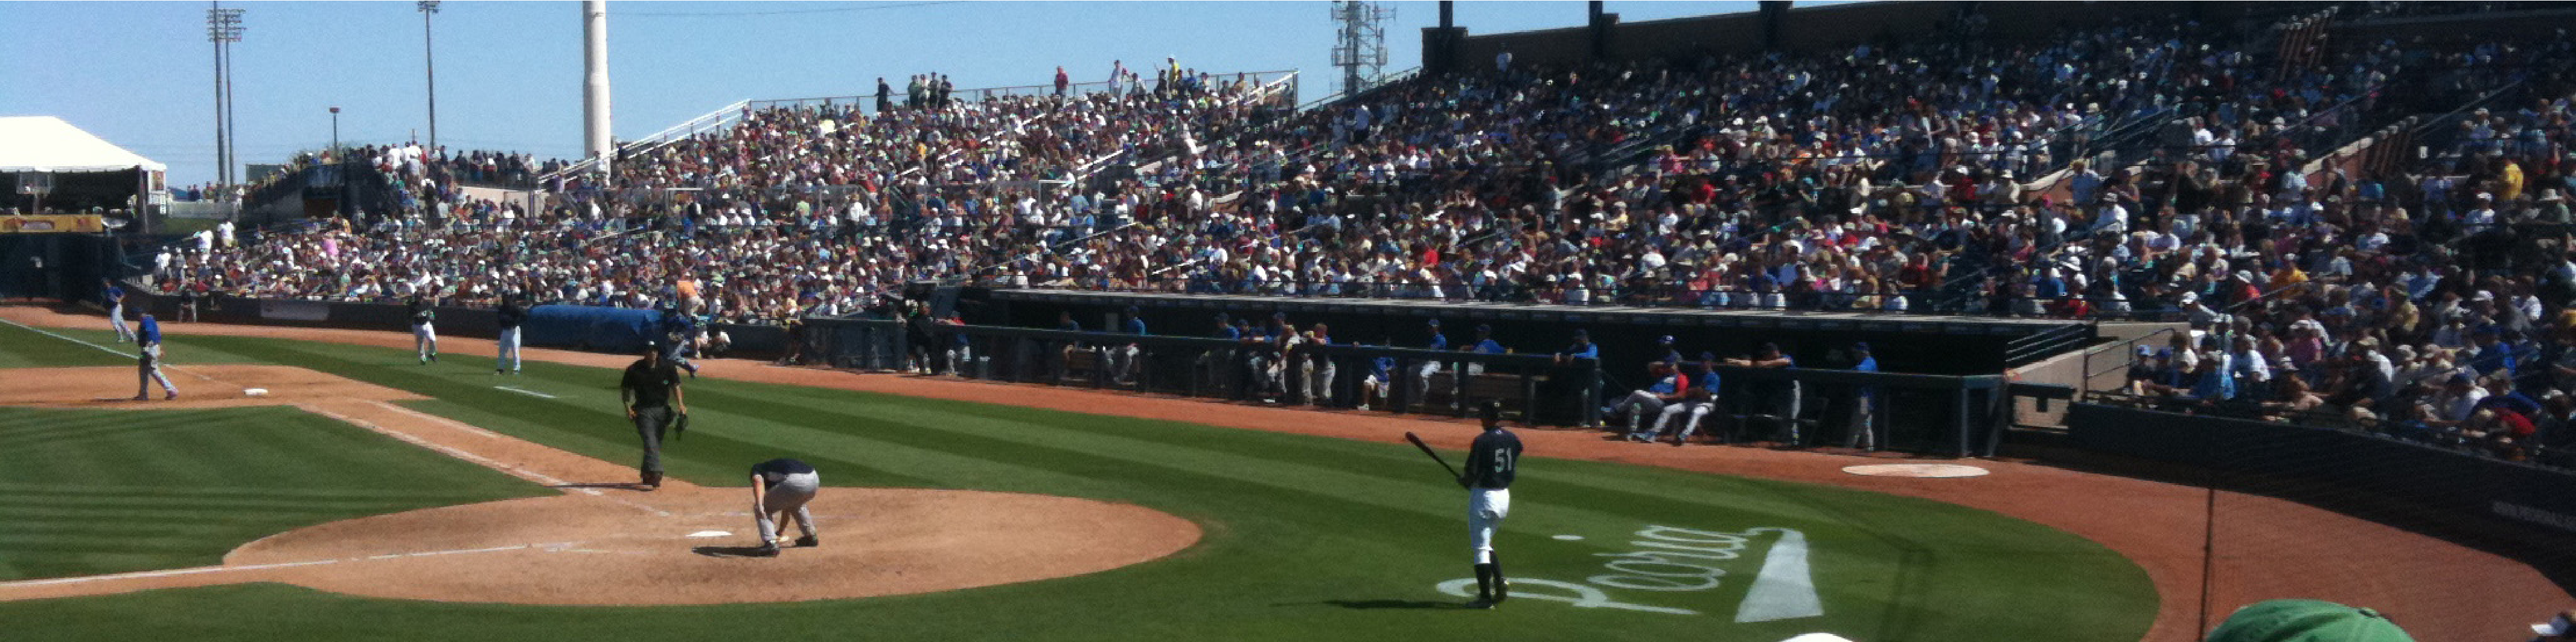
\includegraphics[width=\textwidth]{sampleteaser}
  %%\caption{Seattle Mariners at Spring Training, 2010.}
  %%\Description{Enjoying the baseball game from the third-base
  %%seats. Ichiro Suzuki preparing to bat.}
  %%\label{fig:teaser}
%%\end{teaserfigure}

\received{20 February 2007}
\received[revised]{12 March 2009}
\received[accepted]{5 June 2009}

%%
%% This command processes the author and affiliation and title
%% information and builds the first part of the formatted document.
\maketitle

\section{Introduction}
Dead code, when unaddressed, can be a major problem for a piece of software.
If not eliminated by the compiler, dead code can make a program 
larger, especially if there is a substantial amount of it within a codebase. In addition, dead code 
can make software arbirarily slower, with computational resources being devoted 
to declaring unused variables and empty functions. For these reasons, it is imperative that compilers, at 
a minimum, eliminate chunks of code that are clearly unneeded.

Dead code, as defined in this paper, consists of 
two related, but distinct types of code. Firstly, code can be considered dead if 
it is never actually executed at runtime. For example, code inside of the 'else' portion 
of an if-else block where the condition is always true would be dead. Secondly, a portion of 
code can be considered dead if the computation performed on those lines are never used anywhere else.
For example, a function that is never written to or read from can be considered dead. 

Our project focuses on adding basic dead code elimination strategies into the compiler 
created in the fourth class project. Our goal is to give the compiler support for eliminating
unreachable code in if branches, for loops, and while loops. In addition, the compiler should 
be able to remove unused variables.

\section{Implementation}
In this section, we will outline how we implemented the aforementioned code removal functionality. 

\subsection{If Statements}
We checked the if condition, if the compiled R value was 0, remove the if. If the compiled R value was 1, 
remove the else. Make this sound more compilcated and smart.

\subsection{While Loops}
We checked the condition, if the compiled R value was 0, don't generate a loop at all. If the compiled R value was 1, 
Generate the loop, but heavily shorten the code after it. Make this sound more compilcated and smart.

\subsection{For Loops}
Pretty much the same as the while loop. 

\subsection{Useless Variables}
Hopefully we can get this implemented and talk about it. Worst case, we can just talk about things we considered 
and stuff we tried.

\section{Testing Methodology}
I'm thinking our main metric should be file size in bytes, since this is the main 
purpose of dead code elimination. We can also measure speed as well, but make it clear 
that it isn't as significant. 

\section{Results}
We'll use tables, charts, and other stuff to make our basic testing look fancy.
The better it looks, the more it'll look like we tried.

\begin{table*}
  \caption{Some Typical Commands}
  \label{tab:commands}
  \begin{tabular}{ccl}
    \toprule
    Command &A Number & Comments\\
    \midrule
    \texttt{{\char'134}author} & 100& Author \\
    \texttt{{\char'134}table}& 300 & For tables\\
    \texttt{{\char'134}table*}& 400& For wider tables\\
    \bottomrule
  \end{tabular}
\end{table*}

\section{Conclusion}

We can talk about our results and talk about how the simple examples could 
extend to bigger examples and that big code bases need dead code elim. Blah blah blah.


\end{document}
\endinput
%%
%% End of file `sample-lualatex.tex'.
